
’大学\documentclass[addpoints]{physlabs}

\labtitle{Wave Properties of the Electromagnetic Spectrum}
\labnum{13}
\labnumroman{XIII}
\course{PHYSICS 123 - 183}
\coursesubtitle{Waves and Modern Physics}
\date{\today}

\usetikzlibrary{patterns, patterns.meta, angles, calc, quotes, shapes, shapes.geometric, arrows.meta}

% Commands for tikz
\newcommand\rightAngle[4]{
  \pgfmathanglebetweenpoints{\pgfpointanchor{#2}{center}}{\pgfpointanchor{#3}{center}}
  \coordinate (tmpRA) at ($(#2)+(\pgfmathresult+45:#4)$);
  \draw[white,line width=0.6] ($(#2)!(tmpRA)!(#1)$) -- (tmpRA) -- ($(#2)!(tmpRA)!(#3)$);
  \draw[RubineRed] ($(#2)!(tmpRA)!(#1)$) -- (tmpRA) -- ($(#2)!(tmpRA)!(#3)$);
}
\newcommand\lineend[2]{
  \def\w{0.1} \def\c{30}
  \draw[YellowOrange] (#1)++(#2:\w) to[out=#2-180-\c,in=#2+\c] (#1)
                               to[out=#2+\c-180,in=#2-\c]++ (#2-180:\w);
}

\begin{document}

\maketitle

% PRELAB SECTION
\begin{prelab}

    \filbreak
    \question[1] Using the equation $\lambda=d\sin{\theta}$, derive an expression for $(\Delta\lambda/\lambda)^2$ using the method of error propagation described in \href{https://www.pas.rochester.edu/%7Ephyslabs/manuals/AppendixB.pdf}{\textsl{Appendix B: Error Analysis}} on the Physics Labs website.
    %
    \begin{solution}[7cm]
        
    \end{solution}

    \filbreak
    \question[1] How can you determine the slit separation by observing the interference pattern in this experiment? Explain your reasoning.
    %
    \begin{solution}[3cm]
        
    \end{solution}
    
\end{prelab}

% LAB SECTION
\begin{labsection}

\begin{objective}
    To observe wavelike interference patterns with electromagnetic radiation, and to calculate the wavelengths of a helium-neon laser and a microwave source using the observed interference patterns.
\end{objective}

\begin{theory}
    Since the 17th Century, the prevailing view of the nature of light has changed several times. Isaac Newton described light as a stream of particles (or ``corpuscles''), partly because of its property of straight-line travel. Contemporaries of Newton, such as Christiaan Huygens, argued that light could be explained geometrically as a wave-like phenomenon. In the 19th century, the experimental work of Thomas Young led to the broad acceptance that light consists of waves. And in the 20th century, it was shown that light, or more generally any part of the electromagnetic spectrum, behaves with both particle-like and wave-like properties.
    
    One method of observing the wavelike nature of light is through the interference and diffraction of electromagnetic radiation, as these are fundamentally wavelike behaviors. You will observe interference in laser light and microwaves using a double-slit experiment, and measure diffraction from a single slit.

    \subsection*{Double-Slit Interference}

    If light is incident on a screen with two narrow slits separated by a distance $d$, the slits act as point sources of electromagnetic waves. When the light from the slits is projected onto a screen at a distance $L\gg d$, the light from the slits constructively and destructively interferes at the screen, producing a ``fringe'' pattern of light and dark spots.

    \begin{figure}[ht]
        \centering
        % Diagram of the two-slit interference setup with an inset closeup of the slits.
% Based on https://tikz.net/optics_twoslit/, with some cosmetic adaptations.

\begin{tikzpicture}

    % Closeup view of the two slits
    \begin{scope}[shift={(-6,0)}, scale=1.2]
        \def\L{5.5}       % distance between walls
        \def\l{3.8}       % distance between walls
        \def\H{3.5}       % total wall height
        \def\f{0.9}       % fractional height of projection point
        \def\t{0.15}      % wall thickness
        \def\d{1.6}       % slit distance
        \def\a{0.20}      % slit size
        \def\ang{27}      % angle
        \coordinate (T) at (0,\d/2);
        \coordinate (B) at (0,-\d/2);
        \coordinate (L) at (0,0);
        \coordinate (R) at (\L,0);
        \coordinate (I) at ({\d/2/tan(\ang)},0);

        % LINES
        \draw[photon] (T) --++ (\ang:.8*\l) coordinate (PT) node[midway,below=1,above left=-2] {$r_1$};
        \draw[photon] (B) --++ (\ang:\l) coordinate (PB) node[midway,left=2,below right] {$r_2$};
        \draw[RocBlue,dashed] (T) -- ($(B)!(T)!(PB)$) coordinate (M);
        \draw[black!60,dashed] (L) --++ (\ang:.9*\l) coordinate (PR);
        %\draw[black!60,dashed] (T) --++ (.20*\L,0) coordinate (TR);
        \draw[black!60,dashed] (L) --++ (.6*\L,0) coordinate (LR);
        %\draw[black!60,dashed] (B) --++ (.20*\L,0) coordinate (BR);

        % LINE END
        \lineend{PT}{\ang+70}
        \lineend{PB}{\ang+70}

        % ANGLES
        \draw pic[-latex,"$\theta$",RocBlue,draw=RocBlue,angle radius=18.8,angle eccentricity=1.38 ]
          {angle = B--T--M};
        \draw pic[-latex,"$\theta$",RocBlue,draw=RocBlue,angle radius=22,angle eccentricity=1.25]
          {angle = LR--L--PR};
        \draw pic[-latex,"$\theta$",RocBlue,draw=RocBlue,angle radius=22,angle eccentricity=1.30]
          {angle = LR--I--PB};
        \rightAngle{T}{M}{PB}{0.3}

        % MEASURES
        \draw[latex-latex,black] (-2.4*\t,-\d/2) --++ (0,\d) node[midway,fill=white,inner sep=1.5] {$d$};
        \draw[latex-latex,black] ([shift={({\ang-90}:0.1)}]B) -- ([shift={({\ang-90}:0.1)}]M)
          node[midway,above=1,below right]{$\Delta\ell=d\sin\theta$};

        % WALL
        \fill[gray]
          (0,\d/2-\a/2) rectangle (-\t,-\d/2+\a/2)
          (0,\d/2+\a/2) rectangle (-\t,\H/2)
          (0,-\d/2-\a/2) rectangle (-\t,-\H/2);
    \end{scope}

    % Two slit diagram showing the screen
    \begin{scope}
        \def\L{9}       % distance between walls
        \def\H{3.0}       % total wall height
        \def\f{0.9}       % fractional height of projection point
        \def\ang{atan((\f*\H+\a)/\L/2)} % theta
        \def\t{0.1}      % wall thickness
        \def\d{1.5}       % slit distance
        \def\a{0.20}      % slit size
        \coordinate (T) at (0,\d/2);
        \coordinate (B) at (0,-\d/2);
        \coordinate (L) at (0,0);
        \coordinate (R) at (\L,0);
        \coordinate (P) at (\L,\f*\H/2);
        \coordinate (M) at ($(B)!(T)!(P)$);

        % LINES
        \draw[photon] (T) -- (P) node[midway,above=-1] {$r_1$};
        \draw[photon] (B) -- (P) node[midway,below=3,right=6] {$r_2$}; %right=6,below right=-4
        \draw[dashed] (L) -- (P);
        \draw[dashed,black!60] (L) -- (R);
        \draw[RocBlue,dashed] (M) -- (T);

        % ANGLES
        \draw pic[-,"\footnotesize$\theta$",RocBlue,draw=RocBlue,angle radius=26,angle eccentricity=1.25]
          {angle = B--T--M};
        \draw pic[-,"\footnotesize$\theta$",RocBlue,draw=RocBlue,angle radius=38,angle eccentricity=1.14]
          {angle = R--L--P};
        \rightAngle{T}{M}{P}{0.3}

        % MEASURES
        \draw[latex-latex,black] (0,-0.47*\H) --++ (\L,0) node[midway,fill=white] {$L$};
        \draw[latex-latex,black] (-2.5*\t,-\d/2) --++ (0,\d) node[midway,fill=white] {$d$};
        \draw[|-|,black] ([shift={({\ang-90}:0.1)}]B) -- ([shift={({\ang-90}:0.1)}]M)
          node[midway,above=-1,below right=-1]{\small $d\sin\theta$};
        \draw[latex-latex,black] ([shift={(2.5*\t,0)}]P) -- ([shift={(2.5*\t,0)}]R)
          node[midway,fill=white]{$y$};

        % WALL
        \fill[gray]
          (0,\d/2-\a/2) rectangle (-\t,-\d/2+\a/2)
          (0,\d/2+\a/2) rectangle (-\t,\H/2)
          (0,-\d/2-\a/2) rectangle (-\t,-\H/2)
          (\L,-\H/2) rectangle (\L+\t,\H/2);
        \draw[YellowOrange!80!black, fill=white] (P) circle (0.4*\t) node[above left] {$P$};
    \end{scope}

    % Draw a bounding box around part of the scene:
    \draw[densely dotted] (-0.75,-1.75) rectangle (1.75,1.75);

    % Draw a bounding box around the closeup with connections to the larger
    % drawing to show the inset:
    \draw[densely dotted] (-6.75,-2.5) rectangle (-1.75,3);
    \draw[densely dotted] (-1.75,-2.5) -- (1.75,-1.75);
    \draw[densely dotted] (-1.75,3) -- (1.75,1.75);

\end{tikzpicture}
        \caption{Plane electromagnetic waves incident on two slits of width $a$ and separation $d$ produce an interference pattern on a screen located a distance $L$ from the slits. The inset (left) shows that when $L\gg d$, the rays from the two slits can be treated as parallel.}
        \label{fig: two slit interference}
    \end{figure}

    Figure~\ref{fig: two slit interference} shows a ray diagram of two-slit interference for a monochromatic light source. Light from slit 1 travels a distance $r_1$ to the screen, while light from slit 2 travels a distance $r_2$. The interference conditions at the screen are related to the difference in path lengths $\Delta\ell = r_2-r_1 = d\sin{\theta}$:
    %
    \begin{align}
        d\sin{\theta} &= m\lambda, & &\text{constructive interference},
        \label{eq: two slit maximum}
        \\
        d\sin{\theta} &= \left(m+\frac{1}{2}\right)\lambda, & &\text{destructive interference},
        \label{eq: two slit minimum}
    \end{align}
    %
    where $m=0,\pm1,\pm2,\ldots$
    Consider interference at a point $P$ on the screen, at vertical distance $y$ from the midpoint of the two slits. In the limit where $L\gg d$,
    \begin{equation}\label{eq: two slit approx}
        \sin{\theta} \approx \tan{\theta} = \frac{y}{L}.
    \end{equation}
    Combining eqs.~\ref{eq: two slit maximum} and \ref{eq: two slit approx} gives the vertical position of any interference maximum on the screen:
    %
    \begin{align}\label{eq: two slit y position}
        &\boxed{y_\text{max} = m\frac{\lambda L}{d}}\\ 
        &\hspace{40pt}\text{ where  }m=0,\pm 1,\pm2, \dots \nonumber
    \end{align}
    %
    The intensity pattern on the screen, described by
    %
    \begin{equation}\label{eq: two slit intensity}
        I(\theta) = I_\text{max} \cos^2{\left(\frac{\pi}{\lambda}d\sin{\theta}\right)},
    \end{equation}
    %
    is shown in Fig.~\ref{fig: two slit intensity}. In actuality, eq.~\ref{eq: two slit intensity} does not fully describe the fringe pattern, which (as you will observe) includes the effect of single-slit diffraction.

    \begin{figure}[ht]
        \centering
        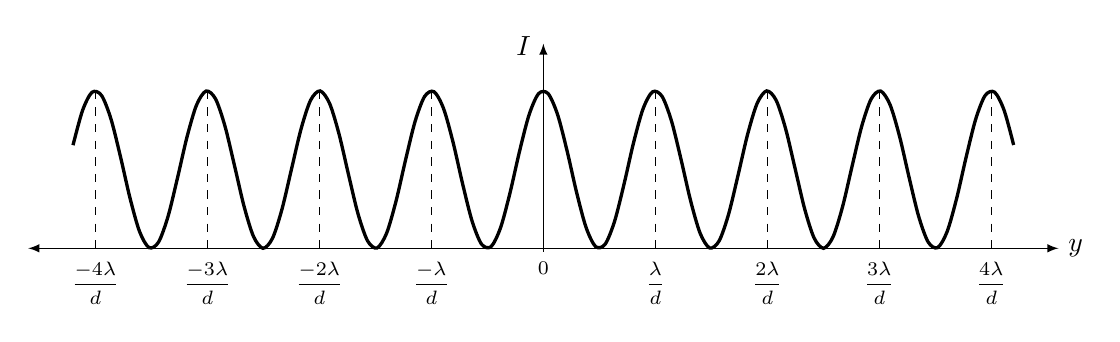
\begin{tikzpicture}
            \def\A{2}
            \def\d{2.25}     % slit distance
            \def\lambd{0.8} % wavelength
            \def\ymax{4*\lambd/\d}
            \def\L{4.0}
            \def\nsamples{100}
            \draw[latex-latex,black] (-4.6*\ymax,0) -- (4.6*\ymax,0) node[right] {$y$};
            \draw[-latex,black] (0,0) -- (0,1.3*\A) node[above=-1, left=1] {$I$};
            \draw[very thick, smooth, samples=\nsamples, variable=\y, domain=-4.2*\ymax:4.2*\ymax] plot(\y, {\A*cos(180*\d*\y/(\lambd*\L))^2});
            \foreach \m in {2, ..., 4} {
                \draw[dashed] (\m*\lambd*\L/\d, \A) -- (\m*\lambd*\L/\d, -0.05) node[below] {\scriptsize $\displaystyle{\frac{\m\lambda}{d}}$};
                \draw[dashed] (-\m*\lambd*\L/\d, \A) -- (-\m*\lambd*\L/\d, -0.05) node[below] {\scriptsize $\displaystyle{\frac{-\m\lambda}{d}}$};
            };
            \draw[dashed] (-\lambd*\L/\d, \A) -- (-\lambd*\L/\d, -0.05) node[below] {\scriptsize $\displaystyle{\frac{-\lambda}{d}}$};
            \draw[dashed] (0, 0) -- (0, -0.05) node[below] {\scriptsize $0$};
            \draw[dashed] (\lambd*\L/\d, \A) -- (\lambd*\L/\d, -0.05) node[below] {\scriptsize $\displaystyle{\frac{\lambda}{d}}$};
        \end{tikzpicture}
        \caption{The two-slit fringe pattern on a screen at a distance $L$ from two slits separated by distance $d$, from eq.~\ref{eq: two slit intensity}.}
        \label{fig: two slit intensity}
    \end{figure}

    \subsection*{Single-Slit Diffraction}

    The wavelike nature of light also causes it to deviate from straight-line motion when it passes around or through an obstacle, such as the single slit of width $a$ shown in Fig.~\ref{fig: single slit diffraction}. The bending and spreading of the waves at the single slit is called diffraction, which produces a characteristic interference pattern distinct from the two-slit fringes discussed above.

    \begin{figure}[ht]
        \centering
        \scalebox{0.95}{% Diagram of single-slit diffraction setup with an inset closeup of the slit.
% Based on https://tikz.net/optics_diffraction/, with some cosmetic adaptations.
\begin{tikzpicture}

    % Closeup view of the single slit
    \begin{scope}[shift={(-7,0)}, scale=1.2]
        \def\L{6.15}      % distance between walls
        \def\l{4.0}       % path length
        \def\H{4.3}       % total wall height
        \def\f{0.9}       % fractional height of projection point
        \def\t{0.15}      % wall thickness
        \def\a{2.5}       % slit distance
        \def\ang{26}      % angle
        \coordinate (T) at (0,\a/2);
        \coordinate (B) at (0,-\a/2);
        \coordinate (L) at (0,0);
        \coordinate (R) at (\L,0);
        \coordinate (I) at ({\a/2/tan(\ang)},0);

        % LINES
        \draw[photon] (T) --++ (\ang:.8*\l) coordinate (PT); 
        %node[midway,below=1,above left=-2] {$r_1$};
        \draw[photon] (B) --++ (\ang:\l) coordinate (PB); %node[midway,left=2,below right=-1] {$r_2$};
        \draw[photon] (L) --++ (\ang:.9*\l) coordinate (PR);
        \draw[dashed] (T) -- (B);
        \draw[RocBlue,dashed] (T) -- ($(L)!(T)!(PR)$) coordinate (M);
        %\draw[black!60,dashed] (T) --++ (.20*\L,0) coordinate (TR);
        \draw[black!60,dashed] (L) --++ (.6*\L,0) coordinate (LR);
        %\draw[black!60,dashed] (B) --++ (.20*\L,0) coordinate (BR);

        % LINE END
        \lineend{PT}{\ang+70}
        \lineend{PR}{\ang+70}
        \lineend{PB}{\ang+70}

        % ANGLES
        \draw pic[-latex,"$\theta$",RocBlue,draw=RocBlue,angle radius=20,angle eccentricity=1.3]
          {angle = B--T--M}; %\contour{white}{}
        \draw pic[-latex,"$\theta$",RocBlue,draw=RocBlue,angle radius=24,angle eccentricity=1.2]
          {angle = LR--L--PR};
        \draw pic[-latex,"$\theta$",RocBlue,draw=RocBlue,angle radius=24,angle eccentricity=1.2]
          {angle = LR--I--PB};
        \rightAngle{T}{M}{PR}{0.3}

        % MEASURES
        \draw[latex-latex,black] (-2.1*\t,0) --++ (0,\a/2) node[midway,fill=white,inner sep=0.1] {$a/2$};
        \draw[latex-latex,black] (-2.1*\t,0) --++ (0,-\a/2) node[midway,fill=white,inner sep=0.1] {$a/2$};
        \draw[latex-latex,black] ([shift={({\ang-90}:0.1)}]L) -- ([shift={({\ang-90}:0.1)}]M)
          node[midway,left=5,below right=-1]{$\displaystyle{\frac{a}{2}\!\sin\theta}$};

        % WALL
        \fill[gray]
          (0,\a/2) rectangle (-\t,\H/2)
          (0,-\a/2) rectangle (-\t,-\H/2);
  \end{scope}

    % Single slit diagram showing the screen
    \begin{scope}
        \def\L{9}         % distance between walls
        \def\H{4.3}       % total wall height
        \def\f{0.95}      % fractional height of projection point
        \def\ang{atan((\f*\H+\a/2)/\L/2)} % theta
        \def\t{0.15}      % wall thickness
        \def\a{2.5}       % slit distance
        \coordinate (T) at (0,\a/2);
        \coordinate (B) at (0,-\a/2);
        \coordinate (L) at (0,0);
        \coordinate (R) at (\L,0);
        \coordinate (P) at (\L,\f*\H/2);
        \coordinate (M) at ($(L)!(T)!(P)$);

        % LINES
        \draw[photon] (T) -- (P); %node[midway,above=-1] {$r_1$};
        \draw[photon] (B) -- (P); %node[midway,below=3,right=6] {$r_2$}; %right=6,below right=-4
        \draw[photon] (L) -- (P);
        \draw[dashed] (T) -- (B);
        \draw[dashed,black!60] (L) -- (R);
        \draw[RocBlue,dashed] (M) -- (T);

        % ANGLES
        \draw pic[-,"\footnotesize$\theta$",RocBlue,draw=RocBlue,angle radius=25,angle eccentricity=1.2]
          {angle = B--T--M};
        \draw pic[-,"\footnotesize$\theta$",RocBlue,draw=RocBlue,angle radius=31,angle eccentricity=1.14]
          {angle = R--L--P};
        \rightAngle{T}{M}{P}{0.3}

        % MEASURES
        \draw[latex-latex,black] (0,-0.47*\H) --++ (\L,0) node[midway,fill=white,inner sep=1] {$L$};
        \draw[latex-latex,black] (-2.1*\t,0) --++ (0,\a/2) node[midway,fill=white,inner sep=0.1] {$a/2$};
        \draw[latex-latex,black] (-2.1*\t,0) --++ (0,-\a/2) node[midway,fill=white,inner sep=0.1] {$a/2$};
        \draw[|-|,black] ([shift={({\ang-100}:0.1)}]L) -- ([shift={({\ang-100}:0.1)}]M)
          node[midway,left=3,below right]{\footnotesize $\displaystyle{\frac{a}{2}\sin\theta}$};
        \draw[latex-latex,black] ([shift={(2.1*\t,0)}]P) -- ([shift={(2.1*\t,0)}]R)
          node[midway,fill=white,inner sep=1]{$y$};

        % WALL
        \fill[gray]
          (0,\a/2) rectangle (-\t,\H/2)
          (0,-\a/2) rectangle (-\t,-\H/2)
          (\L,-\H/2) rectangle (\L+\t,\H/2);
        \draw[YellowOrange!80!black, fill=white] (P) circle (0.4*\t) node[above left] {$P$};
%        \fill[YellowOrange!80!black] (P) circle (0.3*\t) node[right=1,above left=-1] {P};
    \end{scope}

    % Draw a bounding box around part of the scene:
    \draw[densely dotted] (-0.75,-2.25) rectangle (1.75,2.25);

    % Draw a bounding box around the closeup with connections to the larger
    % drawing to show the inset:
    \draw[densely dotted] (-7.75,-2.75) rectangle (-2.5,3.5);
    \draw[densely dotted] (-2.5,-2.75) -- (1.75,-2.25);
    \draw[densely dotted] (-2.5,3.5) -- (1.75,2.25);

\end{tikzpicture}}
        \caption{Plane electromagnetic waves incident on a slits of width $a$ located a distance $L$ from a screen. The inset shows that when $L\gg a$, the rays from every point inside the slit can be treated as parallel.}
        \label{fig: single slit diffraction}
    \end{figure}

    The ray diagram of single-slit diffraction in Fig.~\ref{fig: single slit diffraction} allows us to geometrically derive the diffraction pattern, using an argument first developed by Huygens and refined by French physicist Augustin-Jean Fresnel in the 19th Century. By treating each spatial point in the plane of the slit as a point source of spherical waves, we can construct the condition for interference at the screen. Here we consider the location of the intensity \textsl{minima} in the diffraction pattern, which obey the condition
    %
    \begin{align}
        a\sin{\theta} &= m\lambda, &
        m &= \pm1,\pm2,\ldots &
        &\text{(destructive interference)}.
    \end{align}
    %
    By considering the interference of $n\to\infty$ point sources of spherical waves in the plane of the slit\footnote{A detailed treatment can be found in E. Hecht, \textsl{Optics} (Pearson: 2015), Ch. 10.}, the intensity on the screen as a function of angle can be derived:
    %
    \begin{align}\label{eq: single slit diffracion pattern}
        I(\theta) &= I(0)\sin^2{\left(\frac{\beta}{\beta}\right)},
        &
        \beta &= \frac{\pi a}{\lambda}\sin{\theta},
    \end{align}
    %
    where the intensity minima occur at $\beta=m\pi$, with $m=\pm1,\pm2,\ldots$  The single-slit diffraction pattern is shown in Fig.~\ref{fig: diffraction intensity}.

    \begin{figure}[ht]
        \centering
        \begin{tikzpicture}
            \pgfmathdeclarefunction{sinc}{1}{%
                \pgfmathparse{(#1 == 0 ? 1 : sin(deg(#1)) / #1)}%
            }
            \def\A{5}
            \def\a{3}     % slit width
            \def\lambd{1.1} % wavelength
            \def\ymax{4*\lambd/\a}
            \def\L{4.0}
            \def\nsamples{100}
            \draw[latex-latex,black] (-4.6*\ymax,0) -- (4.6*\ymax,0) node[right] {$y$};
            \draw[-latex,black] (0,0) -- (0,1.1*\A) node[above=-1, left=1] {$I$};
            \draw[very thick, smooth, samples=\nsamples, variable=\y, domain=-4.2*\ymax:4.2*\ymax] plot(\y, {\A*sinc(pi*\a*\y/(\lambd*\L))^2});
            \foreach \m in {2, ..., 4} {
                \draw[dashed] (\m*\lambd*\L/\a, 0) -- (\m*\lambd*\L/\a, -0.1) node[below] {\scriptsize $\displaystyle{\frac{\m\lambda}{a}}$};
                \draw[dashed] (-\m*\lambd*\L/\a, 0) -- (-\m*\lambd*\L/\a, -0.1) node[below] {\scriptsize $\displaystyle{\frac{-\m\lambda}{a}}$};
            };
            \draw[dashed] (-\lambd*\L/\a, 0) -- (-\lambd*\L/\a, -0.1) node[below] {\scriptsize $\displaystyle{\frac{-\lambda}{a}}$};
            \draw[dashed] (0, 0) -- (0, -0.1) node[below] {\scriptsize $0$};
            \draw[dashed] (\lambd*\L/\a, 0) -- (\lambd*\L/\a, -0.1) node[below] {\scriptsize $\displaystyle{\frac{\lambda}{a}}$};
        \end{tikzpicture}
        \caption{The diffraction pattern from a single slit of width $a$.}
        \label{fig: diffraction intensity}
    \end{figure}

    The actual interference pattern from the double slit will be a combination of the fringe pattern and the diffraction from each slit. The combined pattern is described by eq.~\ref{eq: full two slit pattern} and plotted in Fig.~\ref{fig: full two slit pattern}.
    %
    \begin{align}\label{eq: full two slit pattern}
        I(\theta) &= I(0)\sin^2{\left(\frac{\beta}{\beta}\right)}
                         \cos^2{(\delta)},
        &
        \beta &= \frac{\pi a}{\lambda}\sin{\theta},
        &
        \delta &= \frac{\pi d}{\lambda}\sin{\theta}.
    \end{align}

    \begin{figure}[ht]
        \centering
        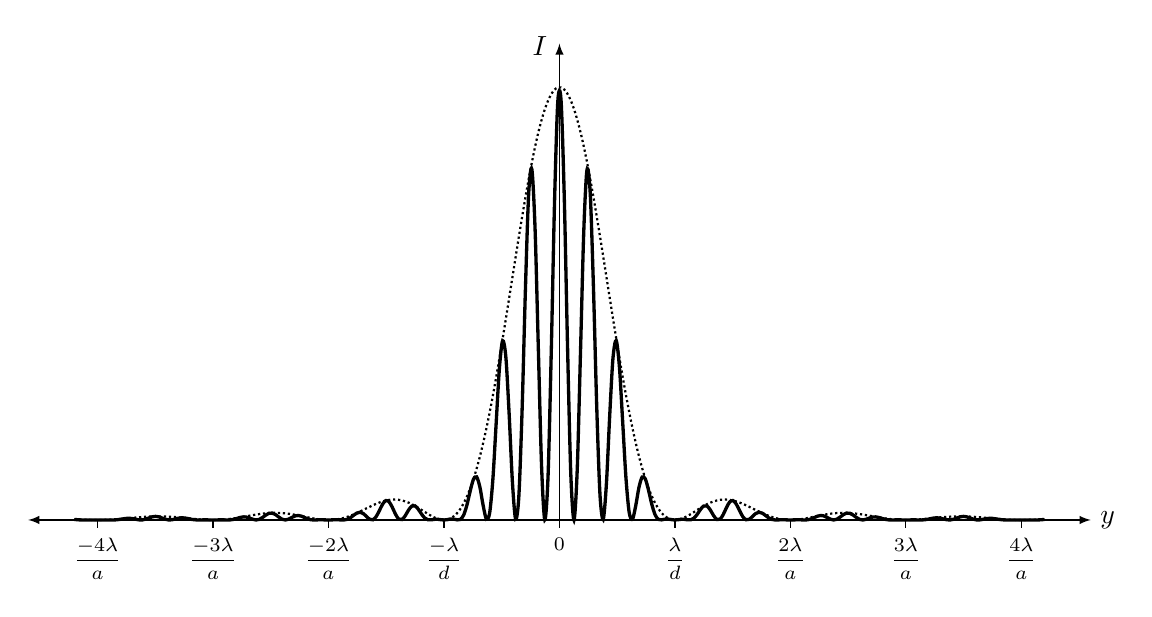
\begin{tikzpicture}
            \pgfmathdeclarefunction{sinc}{1}{%
                \pgfmathparse{(#1 == 0 ? 1 : sin(deg(#1)) / #1)}%
            }
            \def\A{5.5}
            \def\a{3}       % slit width
            \def\d{12}      % slit separation
            \def\lambd{1.1} % wavelength
            \def\ymax{4*\lambd/\a}
            \def\L{4.0}
            \def\nsamples{300}
            \draw[latex-latex,black] (-4.6*\ymax,0) -- (4.6*\ymax,0) node[right] {$y$};
            \draw[-latex,black] (0,0) -- (0,1.1*\A) node[above=-1, left=1] {$I$};
            % Draw the single-slit envelope
            \draw[thick,densely dotted, smooth, samples=\nsamples, variable=\y, domain=-4.2*\ymax:4.2*\ymax] plot(\y, {\A*sinc(pi*\a*\y/(\lambd*\L))^2});
            % Draw the two-slit fringes
            \draw[very thick, smooth, samples=\nsamples, variable=\y, domain=-4.2*\ymax:4.2*\ymax] plot(\y, {\A*sinc(pi*\a*\y/(\lambd*\L))^2*cos(180*\d*\y/(\lambd*\L))^2});
            % Draw some grid points
            \foreach \m in {2, ..., 4} {
                \draw[dashed] (\m*\lambd*\L/\a, 0) -- (\m*\lambd*\L/\a, -0.1) node[below] {\scriptsize $\displaystyle{\frac{\m\lambda}{a}}$};
                \draw[dashed] (-\m*\lambd*\L/\a, 0) -- (-\m*\lambd*\L/\a, -0.1) node[below] {\scriptsize $\displaystyle{\frac{-\m\lambda}{a}}$};
            };
            \draw[dashed] (-\lambd*\L/\a, 0) -- (-\lambd*\L/\a, -0.1) node[below] {\scriptsize $\displaystyle{\frac{-\lambda}{d}}$};
            \draw[dashed] (0, 0) -- (0, -0.1) node[below] {\scriptsize $0$};
            \draw[dashed] (\lambd*\L/\a, 0) -- (\lambd*\L/\a, -0.1) node[below] {\scriptsize $\displaystyle{\frac{\lambda}{d}}$};
        \end{tikzpicture}
        \caption{The observed intensity pattern in a two-slit experiment with slit width $a$ and slit spacing $d=4a$.}
        \label{fig: full two slit pattern}
    \end{figure}
    
\end{theory}

\begin{experiment}

    For the optical measurements in this lab, you will be using a \qty{632.8}{\nano\meter} He-Ne laser. You will mount the slit(s) and the screen on an optical bench to obtain a precise spacing $L$. The setup is shown in Fig.~\ref{fig: interference bench}.

    \begin{figure}[ht]
        \centering
        \begin{tikzpicture}
    % Bench dimensions
    \def\L{6}         % screen-slit distance
    \def\t{0.15}      % bench thickness
    \def\ft{0.4}      % foot width
    \def\hs{1.5}      % screen height
    \def\lw{2}        % laser width
    % Table
    \draw[very thick] (-1.1*\L,0) -- (1.1*\L,0);
    % Optical bench with feet
    \draw[fill=black] (-0.4*\L,\t) rectangle (0.3*\L,2*\t);
    \draw[thick] (\ft-0.4*\L,0) rectangle (2*\ft-0.4*\L,\t);
    \draw[thick] (0.3*\L-2*\ft,0) rectangle (0.3*\L-\ft,\t);
    \draw (-0.1*\L, 0.75*\t) -- (0, -3*\t) node[below right] {optical bench};
    % Screen
    \draw[thick] (\L-2*\t, 0) rectangle (\L+2*\t, 2*\t);
    \draw[fill=gray] (\L-0.5*\t,2*\t) rectangle (\L+0.5*\t, \hs);
    \draw (\L+0.5*\t+0.1, \hs) -- (\L+0.5*\t+0.4, 1.5*\hs) node[above] {screen};
    % Laser with feet and stand
    \draw[thick,fill=gray!20] (-\L, 0.5*\hs) rectangle (-\L+\lw, 0.9*\hs) node[pos=0.5] {laser};
    \draw[thick,fill=gray!20] (-\L, 0.5*\hs) rectangle (-\L+\lw, 0.9*\hs) node[pos=0.5] {laser};
    \draw[thick, fill=black] (-\L+\t, 0.5*\hs) rectangle (-\L+2*\t, 0.5*\hs-0.5*\t);
    \draw[thick, fill=black] (-\L+\lw-\t, 0.5*\hs) rectangle (-\L+\lw-2*\t, 0.5*\hs-0.5*\t);
    \draw[pattern={Lines[angle=45, distance=2mm]}] (-\L-2*\t, 0) rectangle (-\L+\lw+2*\t, 0.5*\hs-0.5*\t);
    % Laser aperture and beam
    \draw[thick,fill=gray!20] (-\L+\lw, 0.65*\hs) rectangle (-\L+\lw+\t, 0.75*\hs);
    \draw[photon] (-\L+\lw+\t, 0.7*\hs) -- (\L-0.5*\t, 0.7*\hs);
    % Slit stand
    \draw[fill=white] (-\t, 1.5*\t) rectangle (\t, 2.5*\t);
    \draw[fill=white] (-0.25*\t, 2.5*\t) rectangle (0, 0.9*\hs);
    \draw (-0.1, 0.9*\hs) -- (-0.5, 1.5*\hs) node[above] {slit};
    \draw[fill=white] (-0.75*\t, 0.6*\hs) rectangle (-0.25*\t, 0.8*\hs);
    % Slide-screen distance
    \draw[latex-latex] (0.01*\L, 0.9*\hs) -- (0.98*\L, 0.9*\hs) node[pos=0.5,fill=white] {$L$};
\end{tikzpicture}
        \caption{The optical bench setup for interference and diffraction measurements.}
        \label{fig: interference bench}
    \end{figure}

    \begin{center}
    \setlength{\fboxsep}{6pt}%
    \setlength{\fboxrule}{2pt}%
    \fbox{\begin{minipage}{0.9\textwidth}
        \color{OrangeRed}
        {\bf CAUTION}: Never look directly into the laser beam or allow it to fall on your eyes. Direct exposure to the beam can cause permanent eye damage. When the laser is turned on, but you are not using it for a measurement, keep the aperture covered with a sheet of paper.
    \end{minipage}}
    \end{center}

    \subsection*{Double Slit Interference}

    \begin{enumerate}
        \item Using a microscope, carefully determine the separation of the two slits, $d$, on the slide. Determine the uncertainty in the measured separation. If necessary, convert your result to centimeters and record your result in Data Table~\ref{data: double slit measurements} in the Postlab exercises.
        \textcolor{red}{-The microscope readings are taken using a vernier scale, which I find most students are unfamiliar with. Is it possible to add some illustrations (like the Appendix 2 provided in Experiment 14) on how to read the vernier scale? This will also be helpful for the next experiment if they know about the vernier scale in advance.}

        Turn the screw in only one direction to avoid mechanical ``backlash'' errors. Your lab assistant will help you. (This measurement does not need to be made first. Since there is only one microscope, you may want to wait a while to avoid the queue.)

        \item Set up the apparatus as shown Fig.~\ref{fig: interference bench}. Install the slide in the holder and place it in front of the laser. Aim the laser at the double slit portion \textcolor{red}{-From my experience, some students don't notice that the slit grating has numbers on itself indicating number of slits}
        of your slide and send the back-reflection from the grating back into the laser cavity. This helps to ensure that the $d$ you measured for the slit separation is the $d$ used in the experiment.

        \item Place the screen at the other end of the table from the laser, maximizing $L$. When the laser is turned on, a series of faint parallel vertical fringes will be seen on the screen. The spacing of the fringe maxima, $y$, depends on the screen-slit length $L$ and the wavelength $\lambda$; see eq.~\ref{eq: two slit y position}.

        \item Sketch the fringes in Graph~\ref{graph: double slit patterns} in the Postlab exercises. Use shaded bars or lines to indicate the bright fringes. The brightest fringe (or maximum) on the screen is called the zero-order fringe, $F_0$ (see also Fig.~\ref{fig: full two slit pattern}). $F_0$ is where the path length between the two slits is the same ($\Delta\ell=0$). The two adjacent bright fringes on each side are the first-order maxima, with a path length difference of one wavelength ($\Delta\ell=\lambda$). The next fringes are the second-order maxima, with a path length difference of two wavelengths ($\Delta\ell=2\lambda$), and so on for higher orders.

        \item Measure the separation $y$ on the screen between neighboring fringes. Be sure that you measure the center-to-center distance rather than the edge-to-edge distance. Note: while you could measure two adjacent fringes, a more accurate method is to measure the separation between six to eight fringes and then divide by the number of fringe spacings, yielding the average separation of two adjacent fringes. Furthermore, because the fringes are not sharp lines, you may want to make several measurements. Record your measurements in Data Table~\ref{data: double slit measurements} in the Postlab exercises.

        \item Finally, measure the distance $L$ from the slits to the screen. Then use $L$, $d$, and $y$ in eq.~\ref{eq: two slit y position} to calculate the wavelength of the laser light, $\lambda$. Compare your experimental value to the known \qty{632.8}{\nano\meter} wavelength of the He-Ne laser. Record your estimate in the Postlab exercises.

    \end{enumerate}

    \subsection*{Single Slit Diffraction}

    In this measurement, you will replace the double-slit slide with a single slit and observe the diffraction pattern independent of the interference fringes.

    \begin{enumerate}
        \item Aim the laser at the single slit portion of the slide. When the laser is aimed properly, an intensity pattern similar to that shown in Fig.~\ref{fig: diffraction intensity} will be visible.

        \item Sketch to scale the appearance of the pattern in Graph~\ref{graph: double slit patterns} in the Postlab exercises. Use shaded bars or lines to indicate the bright fringes. Identify the zero-order fringe in your sketch. Draw the scale of the pattern on your sketch so that you can compare it to the fringes from the double slit.
    \end{enumerate}

    \subsection*{Multiple Slit Interference}

    Use the multiple-slit portion of the grating slide to observe how the interference pattern changes when increasing the number of slits beyond two.

    \begin{enumerate}
        \item Aim the laser at the four-slit portion of the slide. When the laser is aimed properly, an interference pattern will be visible on the screen.

        \item Sketch to scale the appearance of the pattern in Graph~\ref{graph: multiple slit patterns} in the Postlab exercises. Use shaded bars or lines to indicate the bright fringes. Identify the zero-order fringe in your sketch. Draw the scale of the pattern on your sketch so that you can compare it to the single and double slit patterns.

        \item Repeat for the six-slit grating, sketching the fringe pattern to scale in Graph~\ref{graph: multiple slit patterns}.
    \end{enumerate}

    \subsection*{Interference by a Wire Screen}

    Here, we replace the grating slide with a wire mesh, which is just a section from a screen window.

    \begin{enumerate}
        \item Place the wire mesh in the holder. Aim the laser so that it passes through the mesh.

        \item Sketch to scale the appearance of the pattern from the mesh in Figure~\ref{graph: wire mesh}. Explain your observation.

        \item When you are finished using the mesh, please return it to its appropriate location.
    \end{enumerate}

    \subsection*{Double-Slit Interference with a Microwave Source}

    \begin{figure}[ht]
        \centering
        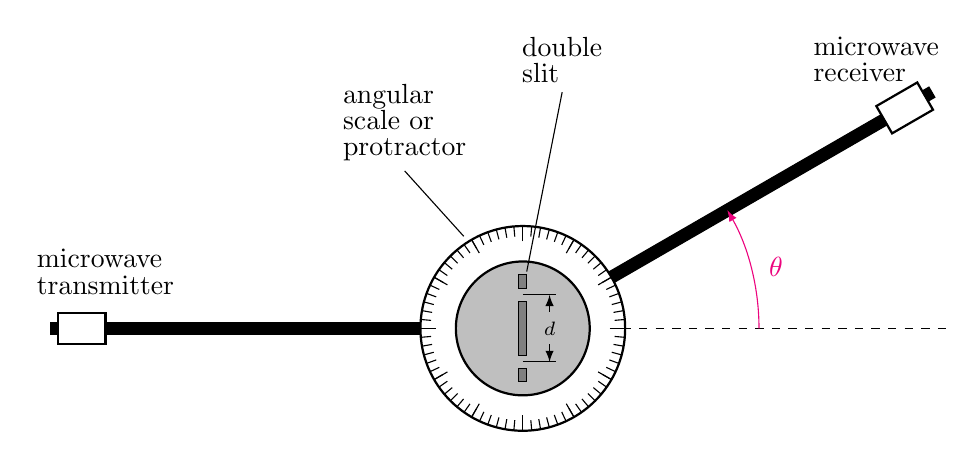
\begin{tikzpicture}
    % Setup dimensions
    \def\L{6}         % screen-slit distance
    \def\t{0.075}     % support beam thickness
    \def\ts{0.05}     % slit thickness
    \def\len{0.6}     % transmitter/receiver length
    \def\wid{0.2}     % transmitter/receiver width
    \def\Rbg{1.3}     % outer radius of the angular scale
    \def\Rsm{0.85}    % inner radius of the angular scale
    %
    % Transmitter arm
    \draw[fill=black] (-\L,-\t) rectangle (0,\t);
    \draw[thick, fill=white] (-\L+0.5*\wid,-\wid) rectangle (-\L+0.5*\wid+\len,\wid) node[above=3, align=left] {microwave\\[-0.25em]transmitter};
    \draw[dashed] (0,0) -- (0.9*\L,0);
    %
    % Receiver arm
    \begin{scope}[rotate around={30:(0,0)}]
        \draw[fill=black] (0,-\t) rectangle (\L,\t);
        \draw[thick, fill=white] (\L-0.5*\wid,-\wid) rectangle
        (\L-0.5*\wid-\len,\wid) node[above=5, align=left] {microwave\\[-0.25em]receiver};
    \end{scope}
    %
    % Angular table
    \draw[thick, fill=white] (0,0) circle (\Rbg);
    \foreach \th in {0, 5, ..., 360}
        \draw[rotate around={\th:(0,0)}] (0.9*\Rbg, 0) -- (\Rbg, 0);
    \foreach \th in {0, 30, ..., 360}
        \draw[rotate around={\th:(0,0)}] (0.85*\Rbg, 0) -- (\Rbg, 0);
    \draw[thick, fill=gray!50] (0,0) circle (\Rsm);
    %
    % Double slit
    \draw[fill=gray] (-\ts, 0.6*\Rsm) rectangle (\ts, 0.8*\Rsm);
    \draw[fill=gray] (-\ts, -0.4*\Rsm) rectangle (\ts, 0.4*\Rsm);
    \draw[fill=gray] (-\ts, -0.6*\Rsm) rectangle (\ts, -0.8*\Rsm);
    \draw (0, -0.5*\Rsm) -- (0.5*\Rsm, -0.5*\Rsm);
    \draw (0,  0.5*\Rsm) -- (0.5*\Rsm,  0.5*\Rsm);
    \draw[latex-latex] (0.4*\Rsm, -0.5*\Rsm) -- (0.4*\Rsm, 0.5*\Rsm) node[pos=0.5, fill=gray!50] {\scriptsize $d$};
    %
    % Labels
    \draw (\ts, 0.85*\Rsm) -- (0.5,3) node[above, align=left] {double\\[-0.25em]slit};
    \draw (-0.75, 0.9*\Rbg) -- (-1.5,2) node[above, align=left] {angular\\[-0.25em]scale or\\[-0.25em]protractor};
    \draw[-latex, RubineRed] (0.5*\L, 0) arc[start angle=0, end angle=30, radius=0.5*\L] node[right=3, pos=0.5] {$\theta$};
\end{tikzpicture}
        \caption{Top view of the setup to measure double-slit interference with a microwave transmitter and receiver.}
        \label{fig: uwave double slit}
    \end{figure}

    In this part of the experiment, you will explore the wave-like nature of a different part of the electromagnetic spectrum, using a microwave transmitter and receiver to determine the wavelength of microwave radiation. Interference maxima and minima will be produced by the double slit, but in contrast to the optical measurement, the separation of the maxima will be measured as an angle rather than as a displacement on a screen. The receiver, shown in Figure~\ref{fig: uwave double slit}, includes a meter to measure the intensity of the radiation received.

    \begin{enumerate}
        \item Use calipers to determine the separation of the centers of the double slit.
        \textcolor{red}{Use calipers to determine the double slit separation. Note: the slit separation is from center of one slit to the other, not the slit width. -I think this may be more clear since students sometimes mix up slit separation and slit width for this part. Also, the double slit is set up using three metal plates. We recommended using $1.5cm$ as slit width. Then, the students can measure the width of the plate in the center to get the slit separation if they add that to $1.5cm$.}
        Record this value, $d$, in Data Table~\ref{data: uwave data} in the Postlab exercises.

        \item Install the double slit on the turntable at the center between the transmitter and receiver horns. \textcolor{red}{Note: The microwave receiver should be placed at the movable end while the transmitter is at the fixed end so the the double slit does not rotate with the receiver.}
        
        \item Align the double slit so that it is normal (perpendicular) to the transmitter horn and centered on the transmitter/receiver axis.
        
        \item Reset the protractor scale so that its \qty{180}{\degree} mark is at the indicator for the transmitter horn.
        
        \item Start with the receiver indicator set at the \qty{0}{\degree} mark. Record the angle (\qty{0}{\degree}) and the receiver meter reading in Data Table~\ref{data: uwave data}. \textcolor{red}{-I remember that when everything is set up accordingly, the receiver actually has \qty{180}{\degree} on its side instead of \qty{0}{\degree}, which shouldn't matter as long as the initial angle is fixed. Is it possible to double check the protractor and rephrase this part to avoid confusions?}
        
        \item Move the receiver \qty{5}{\degree} in one direction and record both the angle and the receiver meter reading in Data Table~\ref{data: uwave data}.
        
        \item  When you find a maximum or a minimum, record both the angle and the receiver meter reading in Data Table~\ref{data: uwave data}.
        
        \item Continue moving the receiver in \qty{5}{\degree} increments in the same direction until you have passed through two maxima. Record both the angle and the receiver meter reading at every position in Data Table~\ref{data: uwave data}.
        
        \item Repeat the measurements to the other side of the \qty{0}{\degree} mark.
    \end{enumerate}
    
\end{experiment}

\end{labsection}

% POSTLAB SECTION
\begin{postlab}

    % Single and double slit questions
    \fullwidth{\subsection*{Double-Slit Interference and Single-Slit Diffraction (\pointsinrange{dblslit} points)}}
    \begingradingrange{dblslit}

    \question[2] Sketch the observed fringes for double slit interference and single slit diffraction in Graph~\ref{graph: double slit patterns}.

    \begin{center}
    \captionsetup{font=normalsize}
    \captionof{graph}{Double-slit and single-slit interference patterns. \label{graph: double slit patterns}}
    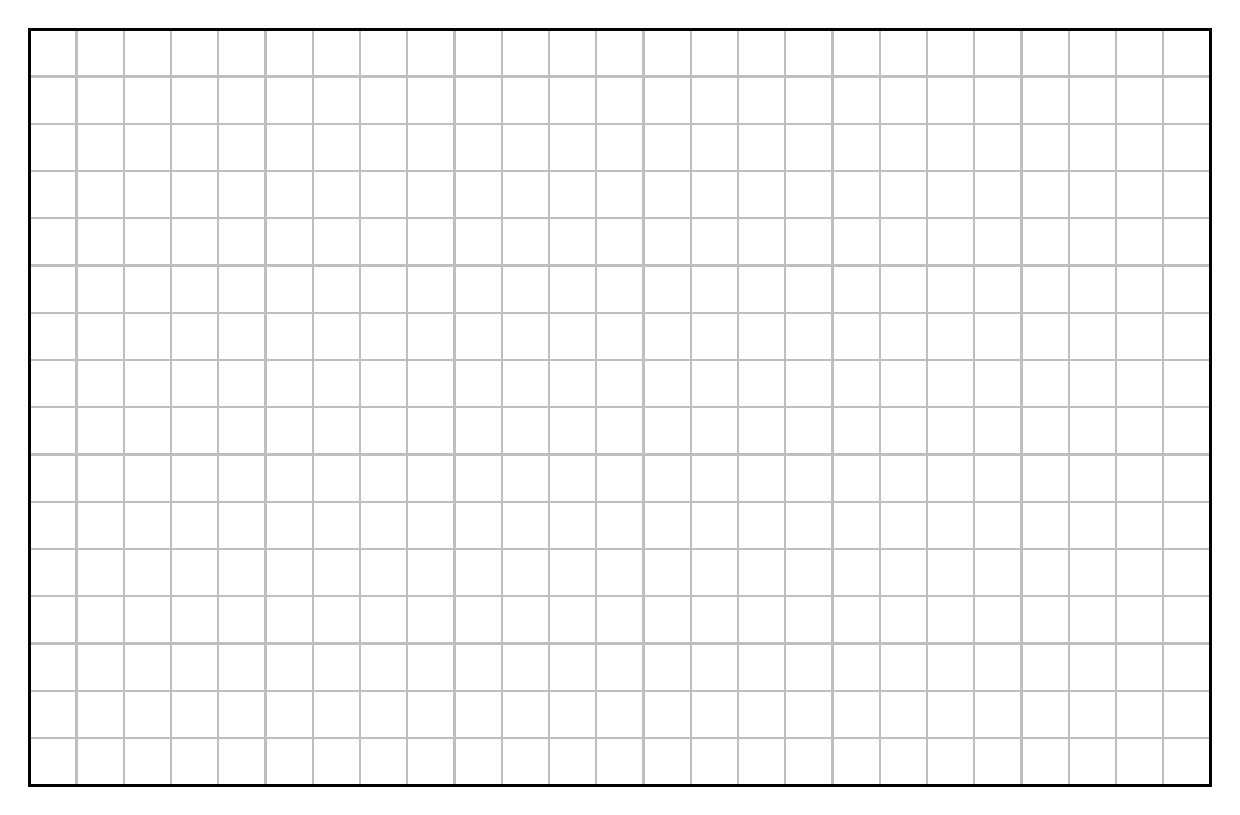
\begin{tikzpicture}
        % Define dimensions
        \def\gridwidth{25}
        \def\gridheight{16}
        \def\spacing{0.6}
        % Draw grid paper on the left
        \begin{scope}[xshift=0cm,yshift=0cm]
            % Major grid lines (thicker)
            \foreach \x in {0,1,...,\gridwidth}
                \draw[gray!50,thick] (\x*\spacing,0) -- (\x*\spacing,\gridheight*\spacing);
            \foreach \y in {0,1,...,\gridheight}
                \draw[gray!50, thick] (0,\y*\spacing) -- (\gridwidth*\spacing,\y*\spacing);
            \draw[black, very thick] (0,0) rectangle (\gridwidth*\spacing,\gridheight*\spacing);
        \end{scope}
    \end{tikzpicture}
    \end{center}

    \question[1] Record the double slit separation $d$, the screen-slit distance $L$, and the average separation between adjacent fringes $y$. Be sure to use the same units for all values.

    \begin{center}
        \renewcommand{\arraystretch}{2}
        \captionsetup{font=normalsize}
        \captionof{data table}{Double-slit measurements. \label{data: double slit measurements}}
        \begin{tabular}{lc>{\centering\arraybackslash}p{3cm}cp{3cm}}
            \hline
            \multicolumn{1}{c}{\textbf{Quantity}} & \multicolumn{2}{c}{\textbf{Measurement}} & \multicolumn{2}{c}{\textbf{Uncertainty}}
            \\
            Double slit separation & $d=$  & & $\Delta d=$ &
            \\
            \cline{3-3}\cline{5-5}
            Screen-slit distance & $L=$ & & $\Delta L=$ &
            \\
            \cline{3-3}\cline{5-5}
            Average fringe separation & $y=$ & & $\Delta y=$ &
            \\
            \cline{3-3}\cline{5-5}
        \end{tabular}
    \end{center}

    \filbreak
    \question[1] Calculate the wavelength $\lambda$ of the He-Ne laser using the observed double slit pattern and eq.~\ref{eq: two slit y position}.
    %
    \begin{solution}[2cm]
    \end{solution}

    \filbreak
    \question[1] Determine the uncertainty $\Delta\lambda$ associated with your experimentally determined wavelength using your estimated uncertainty on $L$, $d$, and $y$. Show your final answer as $\lambda\pm\Delta\lambda$, and compare the result to $\lambda_\text{He-Ne}=\qty{632.8}{\nano\meter}$. Use the expression
    %
    \begin{equation}
        \left(\frac{\Delta\lambda}{\lambda}\right) = \sqrt{\left(\frac{\Delta y}{y}\right)^2 + \left(\frac{\Delta L}{L}\right)^2 + \left(\frac{\Delta d}{d}\right)^2}
    \end{equation}
    %
    \begin{solution}[6cm]
    \end{solution}

    \filbreak
    \question[1] Which parameter of $L$, $d$, and $y$ has the greatest influence on $\Delta\lambda$? Explain your answer.
    %
    \begin{solution}[2.5cm]
    \end{solution}

    \filbreak
    \question[2] Compare the single slit and the double slit fringe patterns. What, if anything, can you say about the relationship between them?
    \textcolor{red}{->may be more clear if ask "similarities or differences" instead of "relationship"}
    %
    \begin{solution}[2.5cm]
    \end{solution}

    \endgradingrange{dblslit}

    % Multiple slit section
    \newpage
    \fullwidth{\subsection*{Multiple Slit Interference (\pointsinrange{mltslit} points)}}
    \begingradingrange{mltslit}

    \filbreak
    \question[2] Sketch the 4-slit and 6-slit interference patterns in Graph~\ref{graph: multiple slit patterns}.

    \begin{center}
    \captionsetup{font=normalsize}
    \captionof{graph}{Multiple slit interference patterns. \label{graph: multiple slit patterns}}
    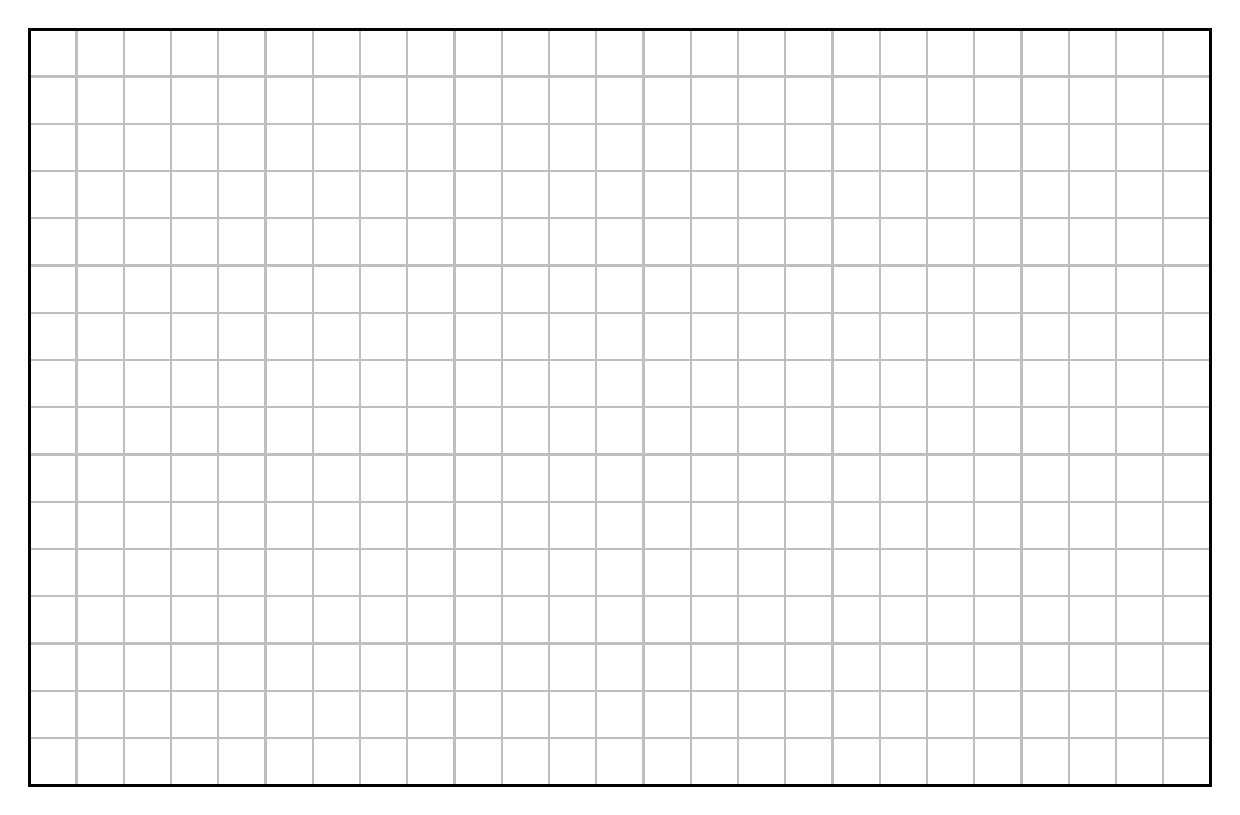
\begin{tikzpicture}
        % Define dimensions
        \def\gridwidth{25}
        \def\gridheight{16}
        \def\spacing{0.6}
        % Draw grid paper on the left
        \begin{scope}[xshift=0cm,yshift=0cm]
            % Major grid lines (thicker)
            \foreach \x in {0,1,...,\gridwidth}
                \draw[gray!50,thick] (\x*\spacing,0) -- (\x*\spacing,\gridheight*\spacing);
            \foreach \y in {0,1,...,\gridheight}
                \draw[gray!50, thick] (0,\y*\spacing) -- (\gridwidth*\spacing,\y*\spacing);
            \draw[black, very thick] (0,0) rectangle (\gridwidth*\spacing,\gridheight*\spacing);
        \end{scope}
    \end{tikzpicture}
    \end{center}

    \filbreak
    \question[1] What happened to the interference pattern as the number of slits increased? Address issues such as brightness, separation, and sharpness.
    %
    \begin{solution}[2.5cm]
        
    \end{solution}

    \filbreak
    \question[1] Without measuring
    \textcolor{red}{using a microscope}, do all the sets of slits on the slide have equal separation? How can you tell \textcolor{red}{from theory and observations}?
    %
    \begin{solution}[2.5cm]
        
    \end{solution}

    \endgradingrange{mltslit}

    % Wire mesh section
    \newpage
    \fullwidth{\subsection*{Interference by a Wire Mesh (\pointsinrange{wiremesh} points)}}
    \begingradingrange{wiremesh}

    \filbreak
    \question[1] Sketch the interference patterns for the wire mesh in Graph~\ref{graph: wire mesh}.

    \begin{center}
    \captionsetup{font=normalsize}
    \captionof{graph}{Interference pattern for the wire mesh. \label{graph: wire mesh}}
    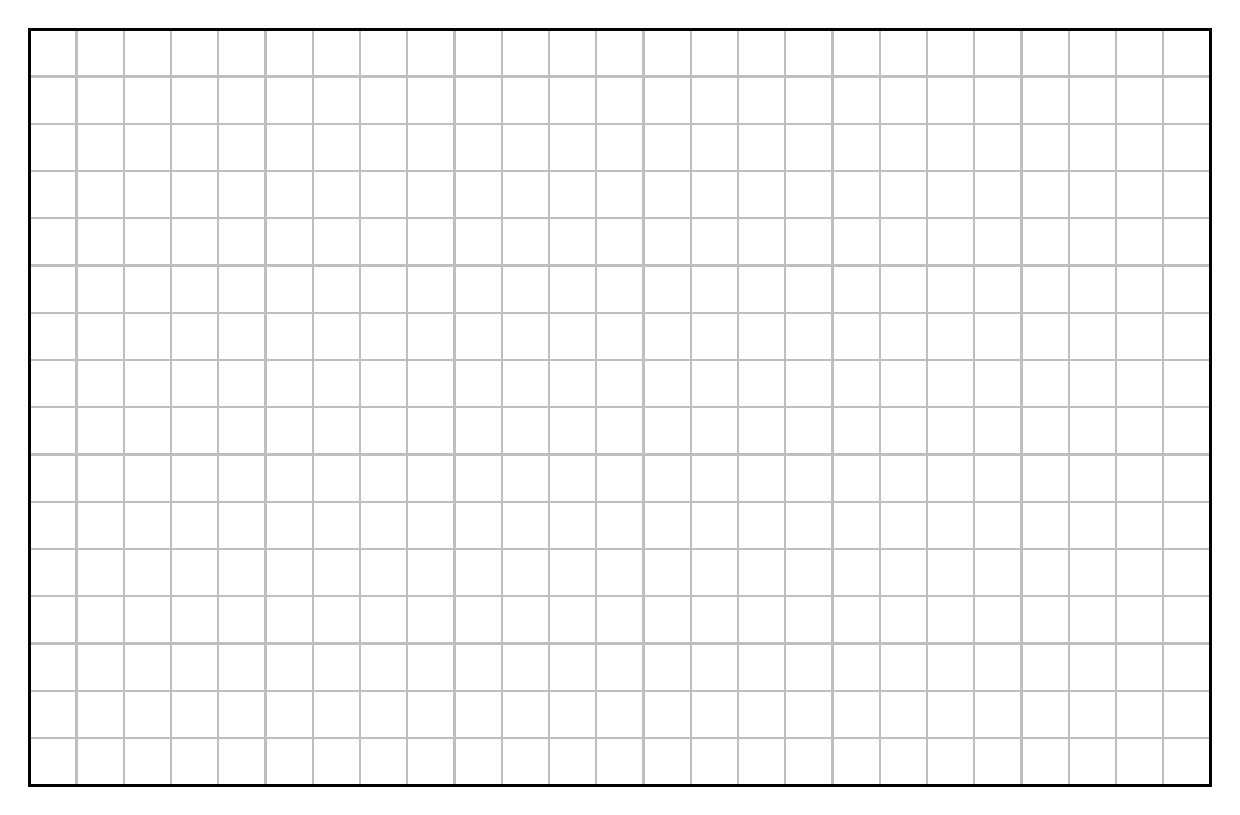
\begin{tikzpicture}
        % Define dimensions
        \def\gridwidth{25}
        \def\gridheight{16}
        \def\spacing{0.6}
        % Draw grid paper on the left
        \begin{scope}[xshift=0cm,yshift=0cm]
            % Major grid lines (thicker)
            \foreach \x in {0,1,...,\gridwidth}
                \draw[gray!50,thick] (\x*\spacing,0) -- (\x*\spacing,\gridheight*\spacing);
            \foreach \y in {0,1,...,\gridheight}
                \draw[gray!50, thick] (0,\y*\spacing) -- (\gridwidth*\spacing,\y*\spacing);
            \draw[black, very thick] (0,0) rectangle (\gridwidth*\spacing,\gridheight*\spacing);
        \end{scope}
    \end{tikzpicture}
    \end{center}

    \filbreak
    \question[1] How can you create an interference pattern similar to the wire screen interference pattern? Explain your reasoning. If necessary, demonstrate or draw a picture showing how to recreate the wire screen interference pattern.
    %
    \begin{solution}[6cm]
        
    \end{solution}

    \endgradingrange{wiremesh}

    % Microwave slit section
    \newpage
    \fullwidth{\subsection*{Microwave Double Slit Measurement (\pointsinrange{uwave} points)}}
    \begingradingrange{uwave}

    \question[1] Record the angle and receiver meter reading at \qty{5}{\degree} increments for as many points as you can obtain data. Record the positions of your maxima and minima as well.
    \textcolor{red}{The last four columns seem confusing to me. Will it be better if they are made into another table that has columns: minima, reading, maxima, reading and indexed rows indicating the order of maxima or minima?}
    \begin{center}
        \renewcommand{\arraystretch}{2}
        \captionsetup{font=normalsize}
        \captionof{data table}{Microwave Double Slit Measurements \label{data: uwave data}}
        \begin{tabular}{|r|c|r|c|>{\centering\arraybackslash}p{2cm}|>{\centering\arraybackslash}p{1.5cm}|>{\centering\arraybackslash}p{2cm}|>{\centering\arraybackslash}p{1.5cm}|}
            \multicolumn{2}{l}{Double slit width:} & \multicolumn{1}{c}{$d=$} &\multicolumn{2}{c}{} & \multicolumn{3}{l}{cm}
            \\
            \cline{4-5}
            \multicolumn{6}{c}{}
            \\
            \hline
            \rowcolor{gray!20}
            $\theta$ [\qty{}{\degree}] & Amplitude & $\theta$ [\qty{}{\degree}] & Amplitude & Minima (angle in \qty{}{\degree}) & Reading (ampl.) & Maxima (angle in \qty{}{\degree}) & Reading (ampl.)
            \\ \hline
             5 & &  -5 & & & & &
            \\ \hline
            10 & & -10 & & & & &
            \\ \hline
            15 & & -15 & & & & &
            \\ \hline
            20 & & -20 & & & & &
            \\ \hline
            25 & & -25 & & & & &
            \\ \hline
            30 & & -30 & & & & &
            \\ \hline
            35 & & -35 & & & & &
            \\ \hline
            40 & & -40 & & & & &
            \\ \hline
            45 & & -45 & & & & &
            \\ \hline
            50 & & -50 & & & & &
            \\ \hline
            55 & & -55 & & & & &
            \\ \hline
            60 & & -60 & & & & &
            \\ \hline
            65 & & -65 & & & & &
            \\ \hline
            70 & & -70 & & & & &
            \\ \hline
            75 & & -75 & & & & &
            \\ \hline
            80 & & -80 & & & & &
            \\ \hline
            85 & & -85 & & & & &
            \\ \hline
            90 & & -90 & & & & &
            \\ \hline
        \end{tabular}
    \end{center}

    \filbreak
    \question[2] Plot the amplitude vs. $\theta$ on the graph in Graph~\ref{graph: uwave slit}. Include units and labels.

    \begin{center}
    \captionsetup{font=normalsize}
    \captionof{graph}{Interference pattern for the wire mesh. \label{graph: uwave slit}}
    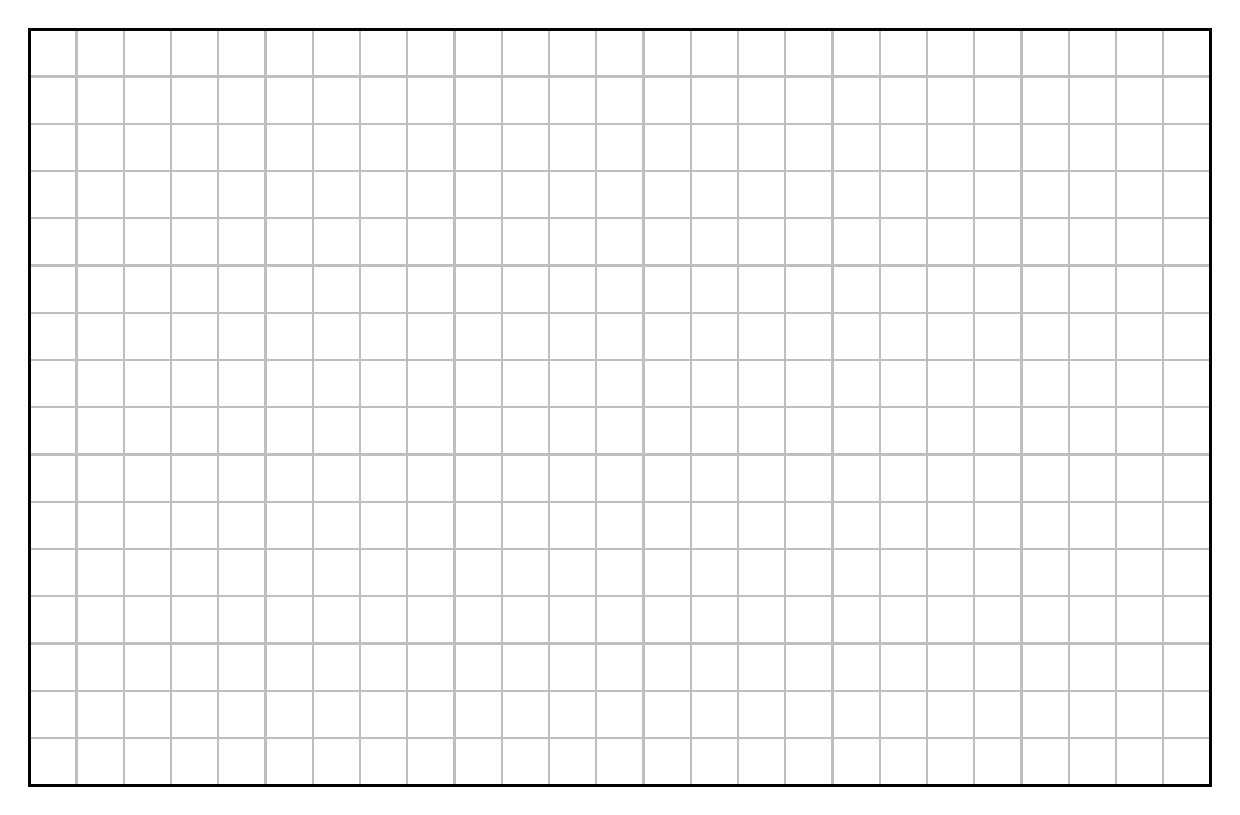
\begin{tikzpicture}
        % Define dimensions
        \def\gridwidth{25}
        \def\gridheight{16}
        \def\spacing{0.6}
        % Draw grid paper on the left
        \begin{scope}[xshift=0cm,yshift=0cm]
            % Major grid lines (thicker)
            \foreach \x in {0,1,...,\gridwidth}
                \draw[gray!50,thick] (\x*\spacing,0) -- (\x*\spacing,\gridheight*\spacing);
            \foreach \y in {0,1,...,\gridheight}
                \draw[gray!50, thick] (0,\y*\spacing) -- (\gridwidth*\spacing,\y*\spacing);
            \draw[black, very thick] (0,0) rectangle (\gridwidth*\spacing,\gridheight*\spacing);
        \end{scope}
    \end{tikzpicture}
    \end{center}

    \filbreak
    \question[1] Using your plot in Graph~\ref{graph: uwave slit}, find the angle between adjacent maxima, $\theta$. You may wish to compute an average value for $\theta$ using the distance between several maxima.
    %
    \begin{solution}[3cm]
        
    \end{solution}

    \filbreak
    \question[1] Using your measurement of $d$, your estimated distance between adjacent maxima $\theta$ , and eq.~\ref{eq: two slit maximum}, calculate the wavelength $\lambda$ of the microwave radiation. Record your uncertainties in Data Table~\ref{data: double slit uwave measurements}.
    %
    \begin{center}
        \renewcommand{\arraystretch}{2}
        \captionsetup{font=normalsize}
        \captionof{data table}{Double-slit microwave measurements. \label{data: double slit uwave measurements}}
        \begin{tabular}{lc>{\centering\arraybackslash}p{3cm}cp{3cm}}
            \hline
            % \multicolumn{1}{c}{\textbf{Quantity}} & \multicolumn{2}{c}{\textbf{Measurement}} & \multicolumn{2}{c}{\textbf{Uncertainty}}
            % \\
            Double slit separation & $d=$  & & $\Delta d=$ &
            \\
            \cline{3-3}\cline{5-5}
            Screen-slit distance & $\theta=$ & & $\Delta \theta=$ &
            \\
            \cline{3-3}\cline{5-5}
            Calculated wavelength & $\lambda=$ & & &
            \\
            \cline{3-3}
        \end{tabular}
    \end{center}

    \filbreak
    \question[1] Determine the uncertainty $\Delta\lambda$ associated with your experimentally determined $\mu$-wave wavelength using your estimated uncertainty on $d$ and $\theta$. Show your final answer as $\lambda\pm\Delta\lambda$. Use the expression
    %
    \begin{equation}
        \left(\frac{\Delta\lambda}{\lambda}\right) = \sqrt{\left(\frac{\Delta d}{d}\right)^2 + \left(\frac{\Delta\theta}{\tan{\theta}}\right)^2},
    \end{equation}
    %
    expressing the uncertainty $\Delta\theta$ in radians. Note that microwaves are typically around a few centimeters in wavelength.
    %
    \begin{solution}[6cm]
    \end{solution}

    \endgradingrange{uwave}
    
\end{postlab}

\end{document}